%%%%%%%%%%%%%%%%%%%%%%%%%%%%%%%%%%%%%%%%%
%
% (c) 2018 by Jennifer Laaser
%
% This work is licensed under the Creative Commons Attribution-NonCommercial-ShareAlike 4.0 International License. To view a copy of this license, visit http://creativecommons.org/licenses/by-nc-sa/4.0/ or send a letter to Creative Commons, PO Box 1866, Mountain View, CA 94042, USA.
%
% The current source for these materials is accessible on Github: https://github.com/jlaaser/pogil-polymers
%
%%%%%%%%%%%%%%%%%%%%%%%%%%%%%%%%%%%%%%%%%

\renewcommand{\figpath}{content}

\begin{activity}[Activity Template]

	\textbf{Focus question:} Put a central question for the students to consider through this exercise here.



\begin{model}[ABC]

	Here is the first model for students to consider

	Here is a second paragraph of text, followed by an image:

	% to include images, put them in the folder specified by figpath and then use:
	\centerline{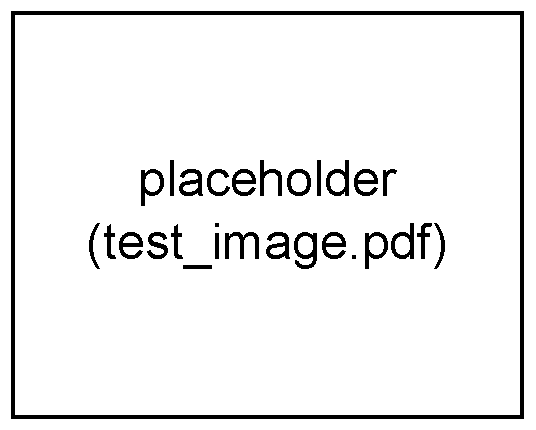
\includegraphics[width=0.5\textwidth]{\figpath/test_image.pdf}}

\end{model}


\begin{ctqs}

	\question First question?
	
		\answerspace{1in}
		
	\question Second question?
	
		\answerspace{1in}
		
	\question Third question?
	
		\answerspace{1in}

\end{ctqs}



\begin{model}[DEF]

	Here is a second model for students to consider.

\end{model}

\begin{ctqs}

	\question First question?
	
		\answerspace{1in}		
	
	\question Second question?
	
		\answerspace{1in}
\end{ctqs}

		
\begin{infobox}
	Here is some useful information that might help the students with the next few critical thinking questions.
	In some cases, it might include an equation:
	\begin{equation*}
		a^2 + b^2 = c^2
	\end{equation*}
	or even more than one equation:
	\begin{equation*}
		x=\frac{-b \pm \sqrt{b^2-4ac}}{2a}
	\end{equation*}
\end{infobox}

\begin{ctqs}

	\question First question?
	
		\answerspace{1in}		
	
	\question Second question?
	
		\answerspace{1in}
\end{ctqs}



\begin{exercises}

	\exercise First exercise
	\exercise Second exercise
	
\end{exercises}


\begin{problems}

	\problem First exercise
	\problem Second exercise
	
\end{problems}


	
\end{activity}